% Appendix Template

\chapter{Appendix of \Cref{chapter:GraphCoupling}}

\minitoc

\section{Proof of \Cref{PCA_graph_coupling}}

\PCAgraphcoupling*

\begin{proof}
We consider the following hierarchical model, for $\nu_{X}, \nu_{Z} \geq n$:
\begin{align*}
    \bm{\Theta}_{X} &\sim  \mathcal{W}(\nu_{X}, \bm{I}_n) \\
    \mathrm{vec}(\X) | \bm{\Theta}_{X} &\sim \mathcal{N}(\bm{0}, \bm{\Theta}_{X}^{-1} \otimes \bm{I}_p) \\
    \bm{\Theta}_{Z} &\sim  \mathcal{W}(\nu_{Z}, \bm{I}_n) \\
    \mathrm{vec}(\Z) | \bm{\Theta}_{Z} &\sim \mathcal{N}(\bm{0}, \bm{\Theta}_{Z}^{-1} \otimes \bm{I}_q) \:.
\end{align*}
With this at hand, the posteriors for $\bm{\Theta}_X$ and $\bm{\Theta}_Z$ can be derived in closed form: 
\begin{align*}
    \bm{\Theta}_{X} | \X &\sim  \mathcal{W}(\nu_{X}+p, \left(\bm{I}_n + \X \X^\top\right)^{-1}) \\
    \bm{\Theta}_{Z} | \Z &\sim  \mathcal{W}(\nu_{Z} + q, \left(\bm{I}_n + \Z \Z^\top\right)^{-1}) \:.
\end{align*}

Keeping terms of $-\mathbb{E}_{\bm{\Theta}_{X}}[\log \mathbb{P}(\bm{\Theta}_{Z} = \bm{\Theta}_{X}| \Z )| \X]$ that depends on $\Z$, one has the optimization problem:
\begin{align*}
    \min_{\Z \in \mathbb{R}^{n \times q}} \quad \frac{\nu_{X}+p}{2}\operatorname{tr}\left(\Z^\top(\bm{I}_n +  \X\X^\top)^{-1}\Z\right) - \frac{\nu_{Z}+q}{2}\log |\bm{I}_n +  \Z\Z^\top|
\end{align*}
Consider the eigendecomposition of the sample covariance matrices: $\X\X^\top = \bm{V D} \bm{V}^\top$ and $\Z\Z^\top = \bm{U \Lambda} \bm{U}^\top$ where $\bm{D}=\operatorname{diag}(\bm{d})$ and $\bm{\Lambda}=\operatorname{diag}(\bm{\lambda})$ such that $d_1 \geq ... \geq d_n$ and $\lambda_1 \geq ... \geq \lambda_n$. Denoting $\gamma = (\nu_{X}+q)/(\nu_{Z}+p)$, we consider the following problem:
\begin{align}
   \min_{\bm{U} \in \mathcal{O}(n), \bm{\Lambda}} \quad & \operatorname{tr}\left(\bm{U} \bm{\Lambda} \bm{U}^\top \bm{V} (\bm{I}_n + \bm{D})^{-1} \bm{V}^\top\right) - \gamma \log |\bm{I}_n + \bm{\Lambda}| \label{eq:optim_eigenvalues_eigenvectors} \\
    \textrm{s.t.} \quad & \bm{\Lambda} \succcurlyeq \bm{0} \label{eq:positive_definite_constraint}\\
    & \operatorname{rank}(\bm{\Lambda}) \leq q \label{eq:rank_constraint}
\end{align}
Note that the above problem is non-convex because of the rank constraint (\ref{eq:rank_constraint}). 

First, we focus on finding the optimal eigenvectors. To that extent, let us denote, $\bm{R} = \bm{U}^\top\bm{V}$. Only the left term in (\ref{eq:optim_eigenvalues_eigenvectors}) depends on $\bm{R}$. The optimization problem for eigenvectors writes:
\begin{align}
   \min_{\bm{R} \in \mathcal{O}(n)} \quad & \operatorname{tr}\left(\bm{R}^\top \bm{\Lambda} \bm{R} (\bm{I}_n + \bm{D})^{-1} \right) \label{eq:optim_eigenvalues_eigenvectors}
\end{align}
The objective (\ref{eq:optim_eigenvalues_eigenvectors}) can be expressed as: $\sum_{(i,j) \in \integ{n}^2} \lambda_i (1 + d_j)^{-1} R_{ij}^2$. Now one can notice that since $\bm{R}$ is orthogonal, $\bm{R} \odot \bm{R}$ is doubly stochastic (\textit{i.e.}\ sum of coefficients on each row and column is equal to one). Therefore thanks to the Birkhoff–von Neumann theorem, there exists $\theta_1, ..., \theta_L \geq 0$, $\sum_{\ell \in \integ{L}} \theta_\ell = 1$ and permutation matrices $\bm{P}_1, ..., \bm{P}_L$ such that:
$$\bm{R} \odot \bm{R} = \sum_{\ell \in \integ{L}} \theta_\ell \bm{P}_\ell$$
where for all $\ell \in \integ{L}$, there exists a permutation $\sigma_\ell$ of $\integ{n}$ such that $P_{\ell,ij} = \ind_{\sigma_{\ell}(i) = j}$ for $(i,j) \in \integ{n}^2$. 

With this at hand, objective (\ref{eq:optim_eigenvalues_eigenvectors}) writes: $\sum_{\ell \in \integ{L}} \theta_\ell \sum_{i \in \integ{n}} \lambda_i (1 + d_{\sigma_\ell(i)})^{-1}$. There exists a permutation $\sigma^\star$ such that the quantity $\sum_{i \in \integ{n}} \lambda_i (1 + d_{\sigma_\ell(i)})^{-1}$ is minimal. Note that the identity permutation \textit{i.e.}\ for $i \in \integ{n}$, $ \sigma(i) = i$ is optimal in this case as the $(\lambda_i)_{i \in \integ{n}}$ and the $(d_i)_{i \in \integ{n}}$ are in decreasing order. Then choosing for $\ell \in \integ{L}$, $\theta_\ell = \ind_{\sigma_\ell = \sigma^\star}$ minimizes the latter quantity. Therefore the solution of (\ref{eq:optim_eigenvalues_eigenvectors}) $\bm{R}^{\star}$ is such that for $(i,j) \in \integ{n}^2$, $R^\star_{ij} = \pm \ind_{\sigma^\star(i)=j}$. Thus an optimum in $\bm{U}$ of $\ref{eq:optim_eigenvalues_eigenvectors}$ is such that $\bm{U}^\star = \bm{V} \bm{R}^\star$. 

Hence $\bm{U} = \bm{V}$, in particular, is optimal. We will choose this $\bm{U}$ in what follows as the sign of the axes do not influence the characterization of the final result in $\Z$ as a PCA embedding. Such a choice gives $\Z \Z^\top = \bm{V} \bm{\Lambda} \bm{V}^\top$. 

Now it remains to find the optimal eigenvalues $(\lambda_i)_{i \in \integ{n}}$. The rank constraint (\ref{eq:rank_constraint}) can be easily dealt with: since the eigenvalues are sorted in decreasing order, the constraint implies that for $i \geq q$, $\lambda_i=0$.  Thus the eigenvalue problem can be formulated in $\mathbb{R}^q$:
\begin{align}
    \min_{\bm{\lambda} \in \mathbb{R}^q} \quad & \bm{\lambda}^\top (\bm{1} + \bm{d})^{-1} - \gamma \bm{1}^\top \log (\bm{1} + \bm{\lambda}) \label{eq:objective_lambda}\\
    \textrm{s.t.} \quad & \forall i \in [q], \quad  \lambda_i \geq 0 , \quad \lambda_1 \geq ... \geq \lambda_q \label{eq:feasibility_lambda}
\end{align}
where (\ref{eq:feasibility_lambda}) accounts for (\ref{eq:positive_definite_constraint}). The above is convex. (\ref{eq:objective_lambda}) is minimized for $\bm{\lambda} = \gamma (\bm{1} + \bm{d}) - \bm{1}$. Taking the feasibility constraint (\ref{eq:feasibility_lambda}) into account one has a solution $\bm{\lambda}^*$ such that:
$$\forall i \in \integ{n}, \quad 
\lambda_i^* = \left\{
    \begin{array}{ll}
        \max(0, \gamma(1 + d_i) - 1) \quad &\mbox{if} \quad i \leq q \\
        0 \quad &\mbox{otherwise} \:.
    \end{array}
\right. $$

Note that this solution is not unique if there are repeated eigenvalues. Notice also that one has the freedom to choose the Wishart prior parameters such that $\gamma=1$. Doing so, the solution satisfies $\Z^\star \Z^{\star \:T} = \bm{V}_{[:,q]} \bm{D}_{[q,q]} \bm{V}^\top_{[q,:]}$. Therefore there exists $\bm{R}$ an orthogonal matrix of size $q$ such that $\Z^{\star} = \bm{V}_{[:,q]}\bm{D}_{[q,q]}^{\frac{1}{2}}\bm{R}$. The latter is the output of a PCA model of $\X$ with $q$ components, which is defined up to a rotation.
\end{proof}

\section{Proof of \Cref{prop:integrability_pairwise_MRF}} \label{proof:lambda_perp_integrability}

\integrabilitypairwiseMRF*

\begin{proof}
$\W \in \mathcal{S}_W$ is the weight matrix of a graph with $R$ connected components $\{C_1, ..., C_R\}$ partitioning $\integ{n}$. Since $k$ is upper bounded by a constant, there exists $M_+ > 1$ that upper bounds $k$. Let $\bm{\mathcal{T}}$ be the adjacency matrix of a spanning forest of $\W$, since each edge of $\W$ is bounded by $n$, one has:
\begin{align}
    \int f_{k}(\X, \W) \lambda_{\mathcal{S}_{C}}(d\X) &= \int \prod_{(i,j) \in \integ{n}^2} k(\mathbf{x}_{i} - \mathbf{x}_{j})^{W_{ij}} \lambda_{\mathcal{S}_{C}}(d\X) \nonumber \\
    &\leq M_+^{n^{3}} \int \prod_{(i,j) \in \integ{n}^2} k(\mathbf{x}_{i} - \mathbf{x}_{j})^{\mathcal{T}_{ij}} \lambda_{\mathcal{S}_{C}}(d\X) \nonumber \\
    &\leq M_+^{n^{3}} \prod_{r \in \integ{R}} \int \prod_{(i,j) \in C_{r}^2} k(\mathbf{x}_{i} - \mathbf{x}_{j})^{\mathcal{T}_{ij}} \lambda_{\mathcal{S}_{C}}(d\X) \:. \label{bound_MRF_product_CC}
\end{align}
Let $r \in \integ{R}$. The spanning tree corresponding to the $r^{th}$ connected component called $\bm{\mathcal{T}}^r$ has exactly $n_r-1$ edges. There exists a leaf node $\ell \in \integ{n}$ of $\bm{\mathcal{T}}^r$ and let $\tilde{\ell}$ be the node linked to it. Consider a bijective map $\sigma \colon C_r \backslash \{\ell\} \to \integ{n_r - 1}$ such that $\sigma(\tilde{\ell}) = 1$ and for $(i,j) \in (C_r \backslash \{\ell\})^2$, $\sigma(i) \leq \sigma(j)$ implies that node $i$ has a shorter path on $\overline{\bm{\mathcal{T}}^r}$\footnote{Symmetrized version \textit{i.e.}\ $\overline{\bm{\mathcal{T}}^r} = \bm{\mathcal{T}}^r + \bm{(\mathcal{T}}^r)^\top$.} to $\ell$ than node $j$. There exists a bijective map $e \colon \integ{2:n_r - 1} \to \integ{n_r - 2}$ such that for $i \in \integ{2:n_R-1}$, $\overline{\bm{\mathcal{T}}^r}_{\sigma^{-1}(i), \sigma^{-1}(e(i))} > 0$ and node $\sigma^{-1}(e(i))$ has a shorter path on $\overline{\bm{\mathcal{T}}^r}$ to node $\ell$ than node $\sigma^{-1}(i)$.

Recall that since $\X \in \mathcal{S}_{C}$ one has: $\sum_{i \in C_r} \mathbf{x}_i = 0$ hence $\mathbf{x}_{\ell} = - \sum_{i \neq \ell} \mathbf{x}_i$. Let us now consider the linear map $\phi^r$ such that:
\begin{align*}
\forall i \in [n_r - 1], \quad \phi^r(\mathbf{x}_i) = \left\{
    \begin{array}{ll}
        \mathbf{x}_{\sigma^{-1}(i)} + \sum_{j \in \integ{n_r - 1}} \mathbf{x}_{\sigma^{-1}(j)} & \mbox{if i = 1}\\
        \mathbf{x}_{\sigma^{-1}(i)} - \mathbf{x}_{\sigma^{-1}(e(i))} & \mbox{otherwise} \:.
    \end{array}
\right.
\end{align*}

We now show that the change of variable $\phi^r$ is a $\mathcal{C}^1$ diffeomorphism by proving that its Jacobian has full rank. Ordering the columns with the map $\sigma$, the latter takes the form:
\[
    \mathbf{J}_{\phi^r} = \left(
    \begin{array}{ccccc}
    2 & 1 & 1 & \dots & 1 \\
      & 1 & 0 & \dots & 0 \\
      &   & \ddots &  \ddots & \vdots \\
      & \Ab &   & \ddots & 0 \\
      &               &   &   & 1
    \end{array}
    \right)
\]
where $\Ab$ is a strictly lower triangular matrix such that for all $i \in \integ{2:n_r-1}$, $A_{ie(i)} = -1$ and for all $t \neq e(i)$, $A_{it}=0$. The above can be factorized as:
\[
\mathbf{J}_{\phi^r} = 
\left(
    \begin{array}{ccccc}
    \alpha_{n_r-1} & \alpha_{n_r-2} & \dots & \alpha_2 & \alpha_1 \\
    0  & 1 & 0 & \dots & 0 \\
    \vdots & \ddots & \ddots & \ddots & \vdots \\
    \vdots & & \ddots & \ddots & 0 \\
    0 & \dots & \dots & 0 & 1
    \end{array}
    \right)^{-1}
\left(
    \begin{array}{ccccc}
    1 & 0 & \dots & \dots & 0 \\
      & 1 & \ddots & & \vdots\\
      & & \ddots & \ddots & \vdots \\
      & \Ab & & \ddots & 0 \\
      & & & & 1
    \end{array}
\right)
\]
where $\alpha_{1}=-1$ and for $\ell > 1$, $\alpha_\ell = \sum_{j < l} \alpha_j\ind_{e(n_r - j)=n_r -\ell} - 1$. With this in place, for $i \in \integ{n_r -1}$, $\alpha_i \neq 0$ in particular $\alpha_{n_r-1} \neq 0$ therefore $|\mathbf{J}_{\phi^r}| \neq 0 $ and $\phi^r$ is a $\mathcal{C}^1$ diffeomorphism. This change of variable yields:
\begin{align*}
\int \prod_{(i,j) \in C_{r}^2} k(\mathbf{x}_{i} - \mathbf{x}_{j})^{\mathcal{T}_{ij}} \lambda_{\mathcal{S}_{C}}(d\X) 
&= \int \bigotimes_{i \in \integ{n_r - 1}} k(\mathbf{y}_i) |\mathbf{J}_{\phi^r}(\mathbf{Y})|^{-1} \lambda_{\mathbb{R}^p}(d\mathbf{Y}) \\
&= |\mathbf{J}_{\phi^r}|^{-1} \prod_{i \in \integ{n_r - 1}} \int k(\mathbf{y}_i) \lambda_{\mathbb{R}^p}(d\mathbf{y}_i)
\end{align*}
using the Fubini Tonelli theorem. The result follows from $\lambda_{\mathbb{R}^p}$-integrability of $k$ and upper bound \ref{bound_MRF_product_CC}.
\end{proof}


\section{Proof of \Cref{prop:posterior_W}}
\label{proof:posterior_limit}

\posteriorW

\begin{proof}
Let $\mathcal{P} \in \{B, D, E\}$, $k$ be a valid kernel (assumptions of \cref{prop:integrability_pairwise_MRF}) with $\K_{X} = (k(\mathbf{x}_{i} - \mathbf{x}_{j}))_{(i,j) \in \integ{n}^2}$ and $\bm{\pi} \in \mathbb{R}_+^{n \times n}$. Let $\W \sim \mathbb{P}_{\mathcal{P},k}^{\varepsilon}(\cdot \: ; \bm{\pi},1)$. Inversion of conditional with Bayes rule gives:
\begin{align}
    \forall \bm{W} \in \mathcal{S}_{W}, \quad \mathbb{P}(\W | \bm{X}) \propto
    \mathcal{C}_{k}^{\varepsilon}(\W)^{-1} f^{\varepsilon}(\X, \W) f_{k}(\X, \W) \mathbb{P}^{\varepsilon}_{\mathcal{P},k}(\W; \bm{\pi}, 1) \label{inversion_Conditional}
\end{align}
where the prior reads:
\begin{align}
    \mathbb{P}_{\mathcal{P},k}^{\varepsilon}(\bm{W}; \bm{\pi}, 1) \propto \mathcal{C}^{\varepsilon}_k(\W) \Omega_{\mathcal{P}}(\W) \prod_{(i,j) \in \integ{n}^2} \pi_{ij}^{W_{ij}} \:.
\end{align}
Hence the joint normalizing constant simplifies such that:
\begin{align}
    \forall \bm{W} \in \mathcal{S}_{W}, \quad \mathbb{P}(\W | \bm{X}) &\propto
    f^{\varepsilon}(\X, \W) \Omega_{\mathcal{P}}(\W) \prod_{(i,j) \in \integ{n}^2} \left(\pi_{ij} k(\mathbf{x}_i - \mathbf{x}_j)\right)^{W_{ij}} \\
    &\xrightarrow[\varepsilon \to 0]{} \Omega_{\mathcal{P}}(\W) \prod_{(i,j) \in \integ{n}^2}  \left(\pi_{ij} k(\mathbf{x}_i - \mathbf{x}_j)\right)^{W_{ij}}
\end{align}
which ends the proof. As a complement, we now explicit the simple forms taken by the posterior limit graph in each case.

\paragraph{$B$-Prior.}
Recall that in this case the prior reads:
\begin{align*}
    \mathbb{P}_{B}^{\varepsilon}(\bm{W}; \bm{\pi},1) &\propto \mathcal{C}_{k}^{\varepsilon}(\bm{W}) \prod_{(i,j) \in \integ{n}^2} \pi_{ij}^{W_{ij}} \ind_{W_{ij} \leq 1} \:.
\end{align*}
Therefore the posterior limit graph has the distribution:
\begin{align*}
    \mathbb{P}_{B}(\W ;\bm{\pi} \odot \bm{K}_{X})
    &= \frac{\prod_{(i,j) \in \integ{n}^2}  \left(\pi_{ij} k(\mathbf{x}_i - \mathbf{x}_j)\right)^{W_{ij}} \ind_{W_{ij} \leq 1}}{\sum_{\W \in \mathcal{S}_{W}} \prod_{(i,j) \in \integ{n}^2}  \left(\pi_{ij} k(\mathbf{x}_i - \mathbf{x}_j)\right)^{W_{ij}} \ind_{W_{ij} \leq 1}} \\
    &= \prod_{(i,j) \in \integ{n}^2}  \left(\frac{\pi_{ij} k(\mathbf{x}_i - \mathbf{x}_j)}{1+\pi_{ij} k(\mathbf{x}_i - \mathbf{x}_j)}\right)^{W_{ij}} \left(\frac{1}{1+\pi_{ij} k(\mathbf{x}_i - \mathbf{x}_j)}\right)^{1-W_{ij}} \ind_{W_{ij} \leq 1} \:.
\end{align*}

This distribution amounts to: $\forall (i,j) \in \integ{n}^2, \quad \W_{ij} \stackrel{\perp\!\!\!\!\perp}{\sim} \mathcal{B}\left( \frac{\pi_{ij} k(\mathbf{x}_i - \mathbf{x}_j)}{1+\pi_{ij} k(\mathbf{x}_i - \mathbf{x}_j)} \right)$.

\paragraph{$D$-Prior.} The prior writes:
\begin{align*}
    \mathbb{P}_{D}^{\varepsilon}(\bm{W}; \bm{\pi}, 1) &\propto \mathcal{C}_{k}^{\varepsilon}(\bm{W}) \prod_{(i,j) \in \integ{n}^2} \pi_{ij}^{W_{ij}} \ind_{W_{i+} = 1} \:.
\end{align*}
The distribution of the posterior limit then becomes:
\begin{align*}
    \mathbb{P}_{D}(\W ;\bm{\pi} \odot \bm{K}_{X}) &= \frac{\prod_{(i,j) \in \integ{n}^2}  \left(\pi_{ij} k(\mathbf{x}_i - \mathbf{x}_j)\right)^{W_{ij}} \ind_{W_{i+} = 1}}{\sum_{\W \in \mathcal{S}_{W}} \prod_{(i,j) \in \integ{n}^2}  \left(\pi_{ij} k(\mathbf{x}_i - \mathbf{x}_j)\right)^{W_{ij}} \ind_{W_{i+} = 1}} \\
    &= \frac{\prod_{(i,j) \in \integ{n}^2}  \left(\pi_{ij} k(\mathbf{x}_i - \mathbf{x}_j)\right)^{W_{ij}} \ind_{W_{i+} = 1}}{\prod_{i \in \integ{n}} \sum_{\ell \in \integ{n}} \pi_{i\ell} k(\mathbf{x}_i - \mathbf{x}_{\ell})} \\
    &= \prod_{(i,j) \in \integ{n}^2} \left(\frac{\pi_{ij} k(\mathbf{x}_i - \mathbf{x}_j)}{\sum_{\ell \in \integ{n}} \pi_{i\ell} k(\mathbf{x}_i - \mathbf{x}_{\ell})}\right)^{W_{ij}} \ind_{W_{i+} = 1} \:.
\end{align*}

This distribution amounts to: $\forall i \in \integ{n}, \quad \W_{i} \stackrel{\perp\!\!\!\!\perp}{\sim} \mathcal{M}\left(1, \left(\frac{\pi_{ij} k(\mathbf{x}_i - \mathbf{x}_j)}{\sum_{\ell \in \integ{n}} \pi_{i\ell} k(\mathbf{x}_i - \mathbf{x}_{\ell})}\right)_{j \in \integ{n}}\right)$.

\paragraph{$E$-Prior.}
In this case the prior reads:
\begin{align*}
    \mathbb{P}_{E}^{\varepsilon}(\bm{W}; \bm{\pi}, 1) &\propto \mathcal{C}_{k}^{\varepsilon}(\bm{W}) \prod_{(i,j) \in \integ{n}^2} \frac{\pi_{ij}^{W_{ij}}}{W_{ij}!} \ind_{W_{++} = n} \:.
\end{align*}
Finally, deriving the distribution of the posterior graph limit:
\begin{align*}
    \mathbb{P}_{E}(\W ;\bm{\pi} \odot \bm{K}_{X}) &= \frac{\prod_{(i,j) \in \integ{n}^2}  (W_{ij}!)^{-1}\left(\pi_{ij} k(\mathbf{x}_i - \mathbf{x}_j)\right)^{W_{ij}} \ind_{W_{++} = n}}{\sum_{\W \in \mathcal{S}_{W}} \prod_{(i,j) \in \integ{n}^2} (W_{ij}!)^{-1} \left(\pi_{ij} k(\mathbf{x}_i - \mathbf{x}_j)\right)^{W_{ij}} \ind_{W_{++} = n}} \\
    &= n! \prod_{(i,j) \in \integ{n}^2} (W_{ij})^{-1} \left(\frac{\pi_{ij} k(\mathbf{x}_i - \mathbf{x}_j)}{\sum_{(\ell,t) \in \integ{n}^2} \pi_{\ell t} k(\mathbf{x}_{\ell} - \mathbf{x}_t)}\right)^{W_{ij}} \ind_{W_{++} = n} \:.
\end{align*}

This distribution amounts to: $\W \sim \mathcal{M}\left(n, \left(\frac{\pi_{ij} k(\mathbf{x}_i - \mathbf{x}_j)}{\sum_{(\ell,t) \in \integ{n}^2} \pi_{\ell t} k(\mathbf{x}_{\ell} - \mathbf{x}_t)}\right)_{(i,j) \in \integ{n}^2}\right)$.
\end{proof}


\section{Towards Capturing Large-Scale Dependencies}\label{sec:towards_large_scale}

In this section, we investigate the ability of graph coupling to faithfully represent the global structure in low dimensions. To gain intuition on the case where the distribution induced by the graph is not degenerate, we consider a proper Gaussian graph coupling model and show its equivalence with PCA. We then provide a new initialization procedure to alleviate the large-scale deficiency of graph coupling when degenerate MRFs are used.

\subsection{Hierarchical Graph Coupling}\label{sec:hierarchical_modelling}

The goal of this section is to show that global structure in SNE-like embeddings can be improved by structuring the CCs' positions. We consider the following hierarchical model for $\Xb$, where $\mathcal{P}_{X} \in \{B,D,E\}$, $k_x$ satisfies the assumptions of \cref{prop:integrability_pairwise_MRF} and $\nu_{X} \geq n$:
\begin{align*}
    \Wb_{X} \sim \mathbb{P}_{\mathcal{P}_X,k_x}^{\varepsilon}(\cdot \: ; \bm{1},1), &\quad \bm{\Theta}_{X} | \Wb_{X} \sim \mathcal{W}(\nu_{X}, \bm{I}_{R}) \\
    \Xb_{C} |\Wb_{X} \sim \mathbb{P}_{k_x}(\cdot \:| \Wb_{X}), &\quad \mathrm{vec}(\Xb_{M}) | \bm{\Theta}_{X} \sim \mathcal{N}\left(\bm{0}, \left(\varepsilon \Ub_{[:R]}  \bm{\Theta}_{X}\Ub^\top_{[R]}\right)^{-1} \otimes \bm{I}_p\right)
\end{align*}
where $\Ub_{R}$ are the eigenvectors associated to the Laplacian null-space of $\overline{\Wb}_{X}$. Given a graph $\Wb_{X}$, the idea is to structure the CCs' relative positions with a full-rank Gaussian model.
The same model is considered for $\Wb_{Z}$, $\bm{\Theta}_{Z}$ and $\Zb$, choosing $\nu_{Z} = \nu_{X} + p - q$ for the Wishart prior to satisfy the assumption of \cref{PCA_graph_coupling}.  With this in place, we aim at providing a complete coupling objective, matching the pairs  $(\Wb_{X},\bm{\Theta}_{X})$ and  $(\Wb_{Z},\bm{\Theta}_{Z})$. The joint negative cross-entropy can be decomposed as follows:
\begin{align}
    &\mathbb{E}_{(\Wb_{X}, \bm{\Theta}_{X})|\Xb}\left[\log \mathbb{P}((\Wb_{Z},\bm{\Theta}_{Z}) = (\Wb_{X},\bm{\Theta}_{X}) | \Zb)\right] \nonumber\\
    &= \mathbb{E}_{\Wb_{X}|\Xb}\left[\log \mathbb{P}(\Wb_{Z} = \Wb_{X} | \Zb)\right] + \label{eq:loss_LW} \\
    & \mathbb{E}_{(\Wb_{X},\bm{\Theta}_{X})|\Xb}\left[ \log \mathbb{P}(\bm{\Theta}_{Z} = \bm{\Theta}_{X}| \Wb_{Z} = \Wb_{X}, \Zb) \right] \label{eq:add_term_Coupling}
\end{align}
where (\ref{eq:loss_LW}) is the usual coupling criterion of $\Wb_X$ and $\Wb_Z$ capturing intra-CC variability while (\ref{eq:add_term_Coupling}) is a penalty resulting from the Gaussian structure on $\mathcal{S}_{M}$. Constructed as such, the above objective allows a trade-off between local and global structure preservation. Following current trends in DR \cite{kobak2021initialization}, we propose to take care of the global structure first \textit{i.e.}\ focusing on (\ref{eq:add_term_Coupling}) before (\ref{eq:loss_LW}). The difficulty of dealing with (\ref{eq:add_term_Coupling}) lies in the hierarchical construction of the graph and the Gaussian precision (see \cref{fig:graphical_model_hierarchical}). We state the following result.

% \begin{wrapfigure}[15]{R}{0.5\textwidth}
% \begin{center}
% \centerline{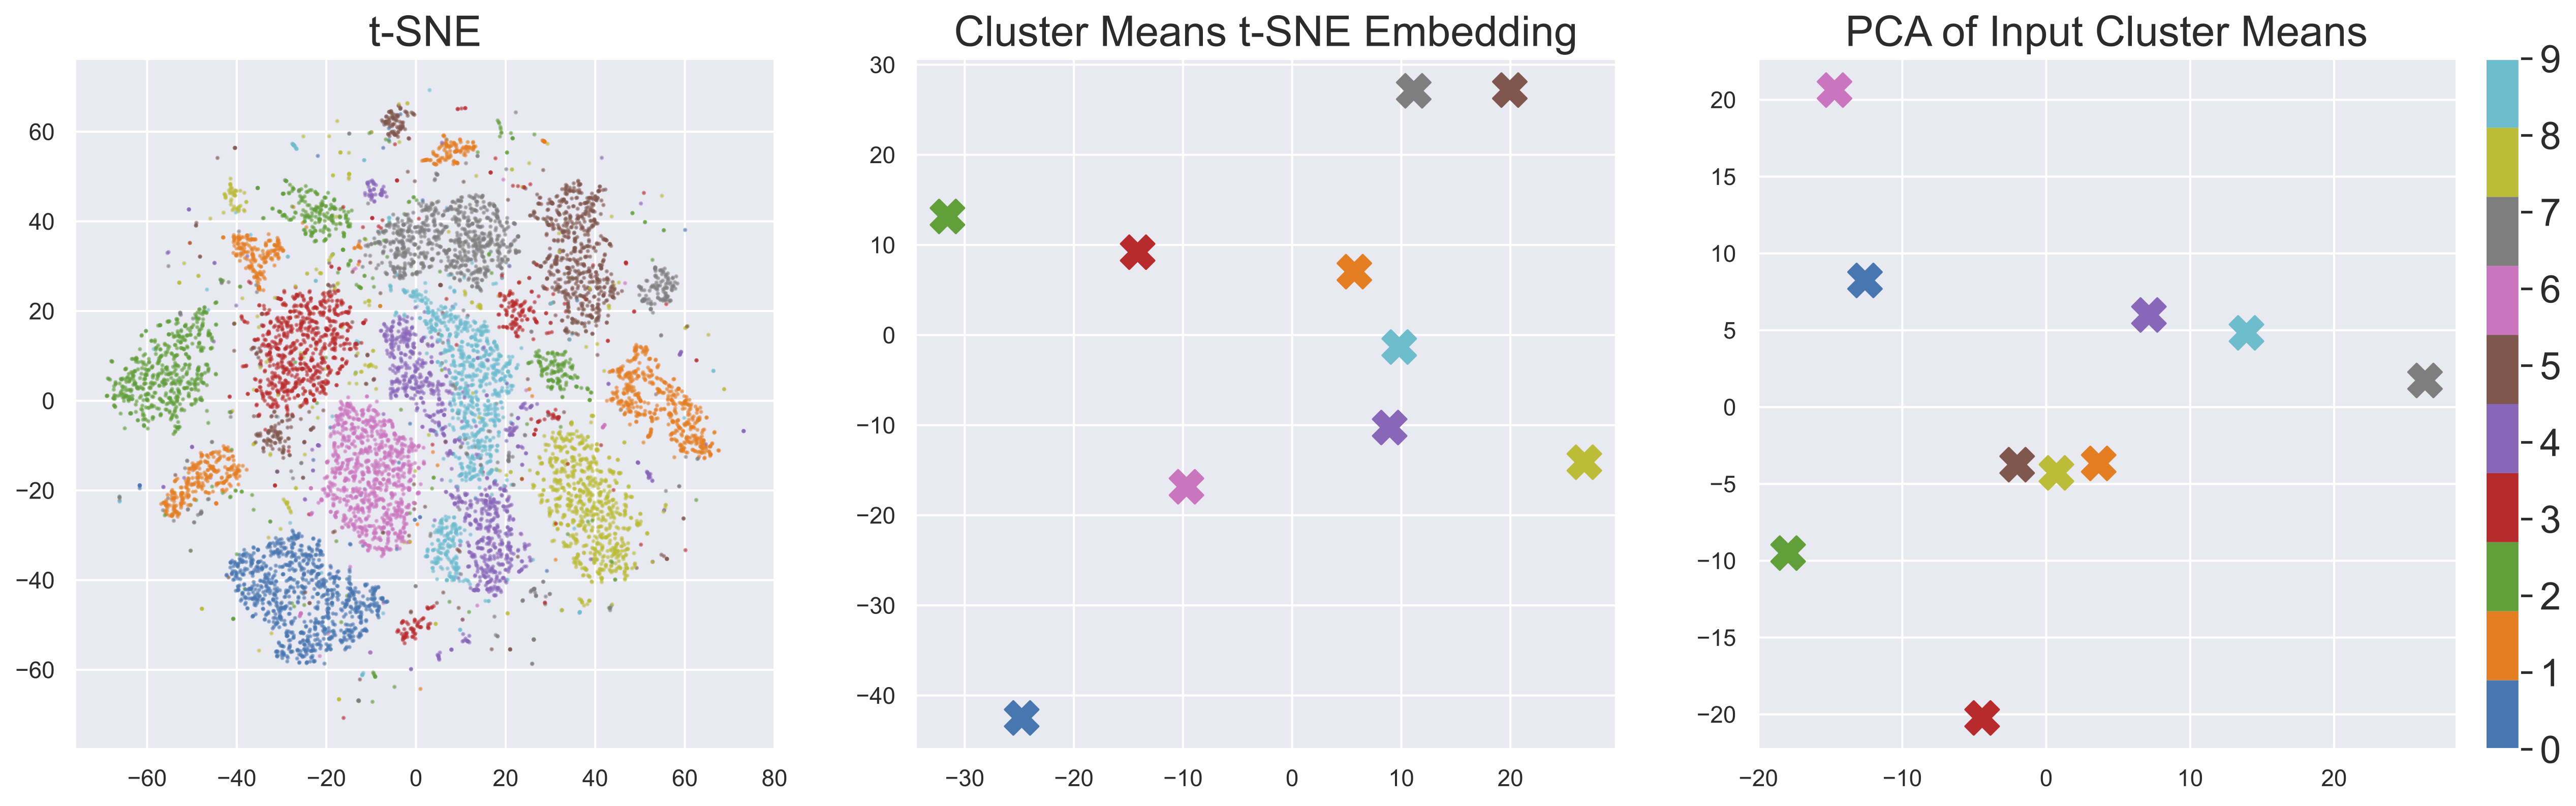
\includegraphics[width=0.5\columnwidth]{figures/GraphCoupling/tSNE_truth.png}}
% \caption{Left: MNIST t-SNE (perp: 30) embeddings initialized with i.i.d $\mathcal{N}(0,1)$ coordinates. Middle: using these t-SNE embeddings, mean coordinates for each digit are represented. Right: we compute a matrix of mean input coordinates for each of the $10$ digits and embed it using PCA. For t-SNE embeddings, the positions of clusters vary across different runs and don't visually match the PCA embeddings of input mean vectors (right plot).}
% \label{fig:tSNE-clusters-truth}
% \end{center}
% \end{wrapfigure}

\begin{corollary}\label{corollary_ccPCA}
Let $\Wb_{X} \in \mathcal{S}_{W}$, $\bm{L} = L(\overline{\Wb}_{X})$ and $\mathcal{S}^q_{M}= (\ker \bm{L}) \otimes \mathbb{R}^q$, then for all $\varepsilon > 0$, given the above hierarchical model, the solution of the problem:
$$\min_{\Zb \in \mathcal{S}^q_{M}} \: -\mathbb{E}_{\bm{\Theta}_{X}| \Xb}\left[ \log \mathbb{P}(\bm{\Theta}_{Z} = \bm{\Theta}_{X}| \Wb_{Z} = \Wb_{X}, \Zb) \right]$$
is a PCA embedding of $\Ub_{[:R]}\Ub_{[R]}^\top\Xb$ where $\Ub_{[:R]}$ are the CCs' membership vectors of $\overline{\Wb}_{X}$.
\end{corollary}

\begin{remark}
Note that while (\ref{eq:loss_LW}) approximates the objective of SNE-like methods when $\varepsilon \to 0$, the minimizer of (\ref{eq:add_term_Coupling}) given by \cref{corollary_ccPCA} is stable for all $\varepsilon$.
\end{remark}

From this observation, we propose a simple heuristic to minimize (\ref{eq:add_term_Coupling}) that consists in computing a PCA embedding of $\mathbb{E}_{\mathbb{P}_{\mathcal{P}_X}(\cdot;\Kb_{X})}\left[ \Ub_{[:R]}\Ub_{[R]}^\top \right]\Xb$. The distribution of the connected components of the posterior of $\Wb_{X}$ being intractable, we resort to a Monte-Carlo estimation of the above expectation. The latter procedure called \textit{ccPCA} aims at recovering the inter-CC structure that is filtered by SNE-like methods. \textit{ccPCA} may then be used as initialization for optimizing (\ref{eq:loss_LW}) which is done by running the DR method corresponding to the graph priors at hand (\cref{sec:retrieving_DR_methods}). This second step essentially consists in refining the intra-CC structure. 

\subsection{Experiments with \textit{ccPCA}}\label{sec:ccPCA}

% \begin{figure*}[t]
% \begin{center}
% \centerline{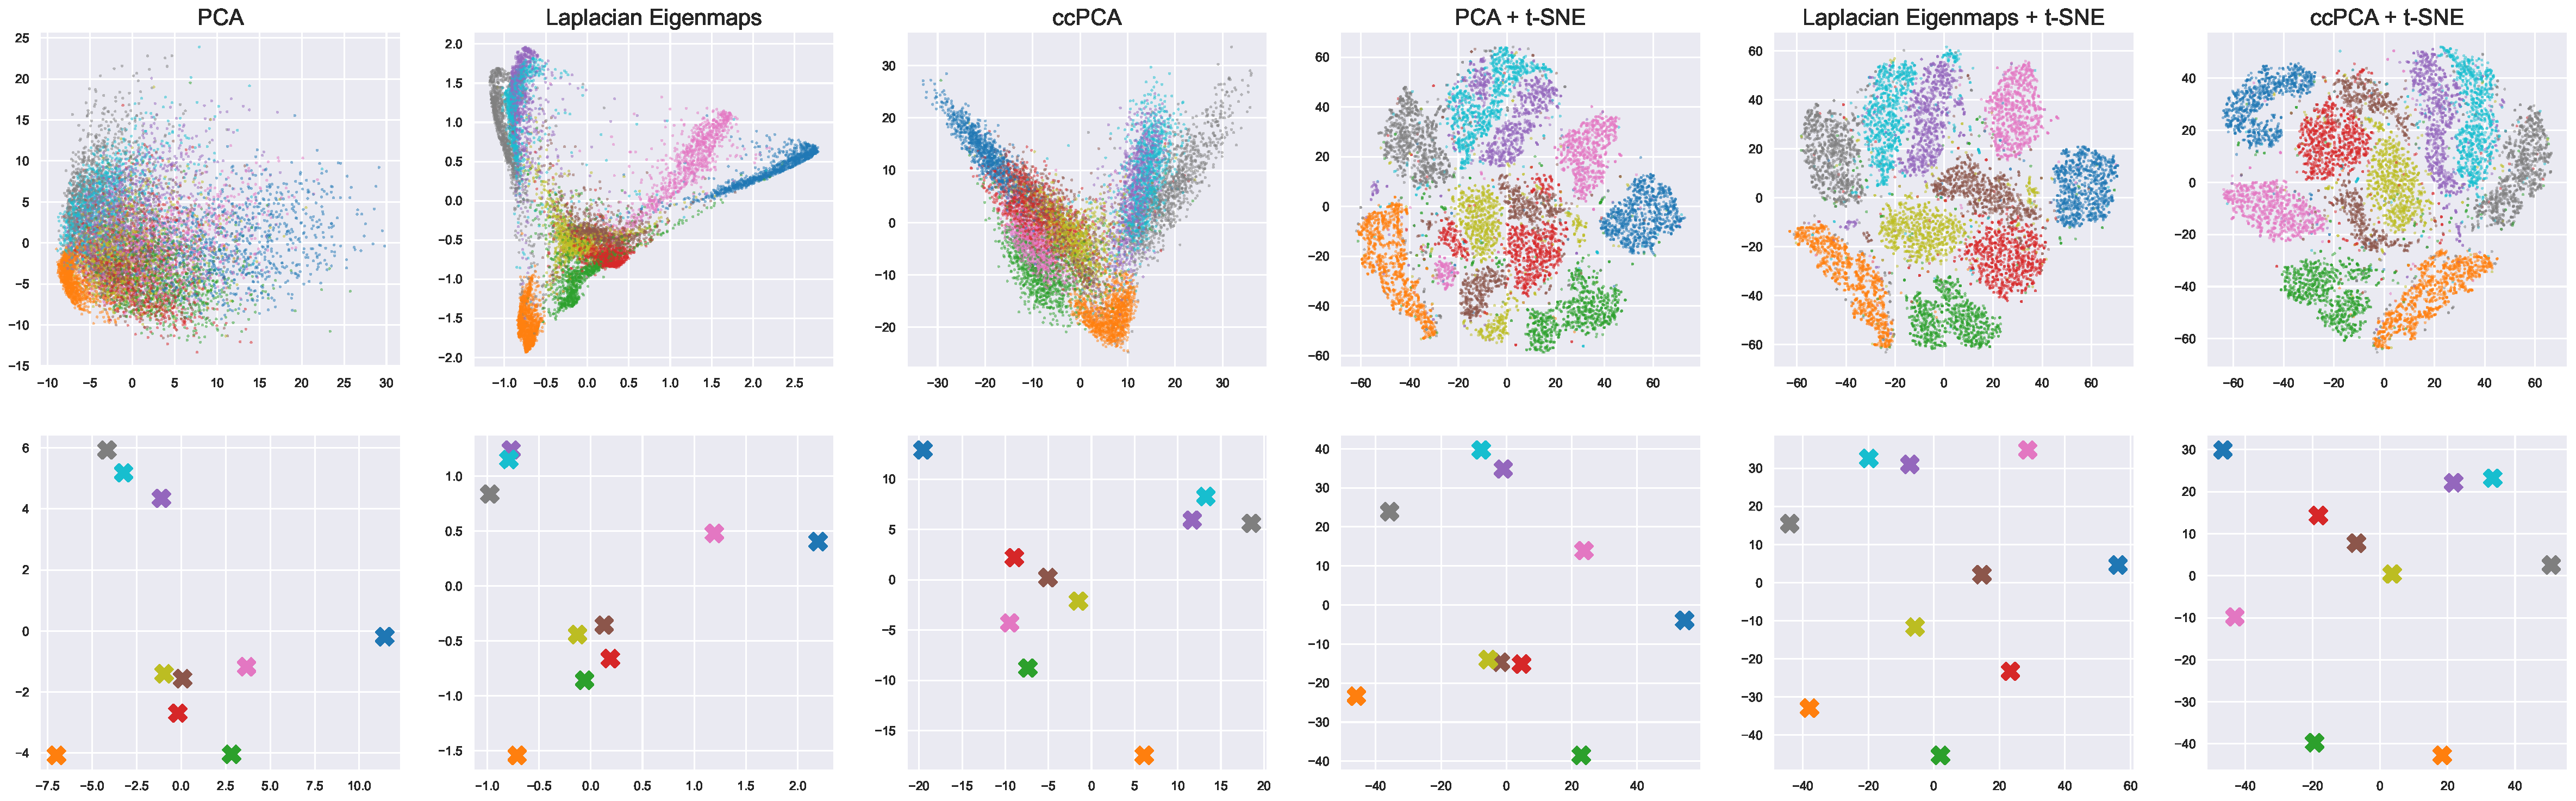
\includegraphics[width=\columnwidth]{figures/GraphCoupling/cluster_positions.png}}
% \caption{Top: MNIST embeddings produced by PCA, Laplacian eigenmaps, \textit{ccPCA} and finally t-SNE launched after the previous three embeddings to improve the fine-grain structure. Bottom: mean coordinates for each digit using the embeddings of the first row. The color legend is the same as in \cref{fig:tSNE-clusters-truth}. t-SNE was trained during $1000$ iterations using default parameters with the openTSNE implementation \cite{polivcar2019opentsne}.}
% \label{fig:methods_embeddings}
% \end{center}
% \vspace{-0.8cm}
% \end{figure*}

\Cref{fig:tSNE-clusters-truth} shows that a t-SNE embedding of a balanced MNIST dataset of 10000 samples \cite{deng2012mnist} with isotropic Gaussian initialization performs poorly in conserving the relative positions of clusters. As each digit cluster contains approximately $1000$ points, with a perplexity of $30$, sampling an edge across digit clusters in the graph posterior $\mathbb{P}_{\mathcal{P}_X}(\cdot;\Kb_{X})$ is very unlikely. Recall that the perplexity value \cite{maaten2008tSNE} corresponds to the approximate number of effective neighbors of each point. Hence images of different digits are with very high probability in different CCs of the graph posterior and their CC-wise means are not coupled as discussed in \cref{sec:interpretations}. To remedy this in practice, PCA or Laplacian eigenmaps are usually used as initialization \cite{kobak2021initialization}. 

These strategies are tested (\cref{fig:methods_embeddings}) together with \textit{ccPCA}. This shows that 
\textit{ccPCA} manages to retrieve the digits that mostly support the large-scale variability as measured by the peripheral positioning of digits $0$ (blue), $2$ (green), $6$ (pink) and $7$ (grey) given by the right side of \cref{fig:tSNE-clusters-truth}. Other perplexity values for \textit{ccPCA} are explored in appendix \ref{sec:other_perp} while the experimental setup is detailed in appendix \ref{sec:setup_exp}. In appendix \ref{sec:quantitative_evaluation}, we perform quantitative evaluations of \textit{ccPCA} for both t-SNE and UMAP on various datasets using K-ary neighborhood criteria. We find that using \textit{ccPCA} as initialization is in general more reliable than PCA and Laplacian eigenmaps for preserving global structure using both t-SNE and UMAP. 

Compared to PCA, \textit{ccPCA} manages to aggregate points into clusters, thus filtering the intra-cluster variability and focusing solely on the inter-cluster structure. Compared to Laplacian eigenmaps which perform well at identifying clusters but suffer from the same deficiency as t-SNE for positioning them, \textit{ccPCA} retains more of the coarse-grain structure. These observations support our unifying probabilistic framework and the theoretical results about the MRF degeneracy which are the leading contributions of this article. The \textit{ccPCA} initialization appears as a first stepping stone towards more grounded DR methods based on the probabilistic model presented in this article.